\chapter{Knowledge-Graph-based Question Generation Pipeline}
\label{chap:construction}

This chapter presents a framework for turning a set of clinical guideline documents into a queryable Knowledge Graph, and for using that graph as a controlled source for generating questions. The four-stage architecture is not specific to diabetes, although the schema, extraction rules, canonical entities, and normalisation procedures used in this thesis are configured for the diabetes guideline corpus.

The chapter follows the same order the pipeline runs in. Section~\ref{sec:corpus} describes the corpus: which documents are used and why. Section~\ref{sec:ingestion} presents the document structuring stage, in which each document is parsed into typed 
element records with page-level provenance. Section~\ref{sec:schema} 
defines the graph model — the node types, relation types, and 
formal properties of the graph. Section~\ref{sec:extraction} 
describes the dual-layer approach to identifying entities and 
relations in the preprocessed records. Section~\ref{sec:normalisation} 
explains how extracted records are deduplicated, unit-normalised, 
and integrated into a single graph. Section~\ref{sec:questions} 
describes how the finished graph is used as a controlled source 
for question generation.

\section{Overview and Objectives}
\label{sec:overview}

The goal of this work is to build a Knowledge Graph that combines several diabetes guidelines into one structured, queryable representation, and to use that graph to generate questions automatically. Eight documents from four organisations are used, covering diagnosis, screening, glycaemic targets, pharmacological management, and monitoring across both Type~1 and Type~2 diabetes. The pipeline is organised into four stages: ingestion, extraction, normalisation, and question generation. This four-stage architecture is not inherently specific to diabetes, but its implementation in this thesis is configured for the diabetes guideline corpus. This includes publisher-specific document-structuring rules, the Knowledge Graph schema, clinical extraction patterns and canonical entities, unit-normalisation procedures, and the relation-to-question mappings. Applying the same architecture to another clinical domain would therefore require adapting these domain- and corpus-specific components. Diabetes guidelines are used as the test domain mainly because they are structurally messy in different ways depending on the publisher, which meant the pipeline had to be tested against a real spread of formats, not one clean case.

This objective breaks down into three concrete reasons for building the graph in the first place.

\paragraph{Cross-guideline comparison}
Once each guideline's content is represented as typed nodes and edges, queries can compare positions across organisations, for example by identifying guidelines that specify the same normalised glycaemic target or recommend the same drug as first-line therapy. Numerical targets are kept organisation-specific and are compared only after unit normalisation, as described in Section~\ref{sec:unit-normalisation}. The resulting cross-guideline comparisons for the diabetes corpus are reported in Chapter~\ref{chap:evaluation}.

\paragraph{Structured accessibility of clinical knowledge }
Guidelines are written for clinicians to read, not for software to parse \cite{peleg2013}. Everything is embedded in prose, numbered lists, and tables, none of which is machine-readable on its own; Section~\ref{sec:bg-ie} discusses this in more depth. Converting that content into a property graph is what makes it possible to query and visualise it, not just search it as text \cite{li2020,harnoune2021}.

\paragraph{Question generation for clinical education }
Once the guideline content sits in a graph, question generation can work directly off graph edges, without needing unstructured passages \cite{guo2024,bi2020}. Selected clinical and cross-guideline edges represent statements extracted from or derived from the source guidelines and can be used as anchors for questions at several difficulty levels, which is useful for building learning or assessment material. The question types used here are defined in Chapter~\ref{chap:background}.

\subsection*{Challenges}

The construction of a multi-guideline knowledge graph introduces five challenges that do not arise in a single-source setting.

Challenge~1 is structural heterogeneity. Because the guidelines come
from distinct publication workflows, there is no uniform document
structure. While some publishers provide clean Unicode text, others
introduce extraction artefacts such as missing whitespace. A fixed
document-structuring procedure therefore cannot be applied unchanged
across the entire corpus. The framework must accommodate
publisher-specific structural differences while producing the same
typed intermediate representation for downstream processing. The
specific repair procedures required for the diabetes corpus are
described in Chapter~\ref{chap:evaluation}.

Challenge~2 is terminological variation. The same clinical idea may be worded differently across organisations. For example "type~2 diabetes" versus "non-insulin-dependent diabetes mellitus" for the same condition. If these forms are kept
as separate identities, relations that should meet at one node are
split across several nodes. The graph therefore needs a canonical form
for such variants before cross-guideline queries are meaningful.

Challenge~3 is unit inconsistency. The guidelines do not consistently use the same measurement units.  A numerical comparison is useless if
the values are not first put on the same scale. A fasting plasma glucose
threshold may be written as 126~mg/dL in one representation and
7.0~mmol/L in another. The numbers look different even though conversion
places them at the same threshold. Cross-guideline comparison therefore
requires unit normalisation before numerical targets are compared.

Challenge~4 is controlling information the language model
introduces beyond what the input actually states. Clinical guideline
text is safety-sensitive: an invented drug indication or a fabricated
contraindication would misrepresent an actual clinical guideline, which
is a more serious failure mode than in general-purpose text generation
\cite{huang2025}. The risk is not limited to entity extraction. In
question generation, a graph anchor may specify an HbA1c threshold without specifying a patient age. A generated vignette that introduces a numerical age has therefore added information not contained in the anchor.
This risk is why the extraction and question-generation stages
(Sections~\ref{sec:extraction} and~\ref{sec:questions}) are built the
way they are: the language model is instructed to classify or rephrase
information already present in the structured input rather than
introduce additional clinical facts, and its output is checked against
that input wherever possible. 

Challenge~5 is entity scoping. Some concepts should be shared across the
whole graph, while others must retain the organisation that stated them.
A Drug such as metformin can be represented by one global node even when
several guidelines mention it. A numerical target is different. If ADA
and IDF both state an FPG threshold of 7.0~mmol/L, the two target nodes
remain separate because they represent independent guideline statements.
Their agreement is represented by an \textsc{equivalent\_to} edge rather
than by merging the nodes. This distinction is fixed by the schema and
carried through deduplication and normalisation.

\subsection*{Contributions}

The pipeline consists of four main technical components.

The first is separating entity types into two extraction layers before any extraction runs. This differs from the hybrid approaches of running rules first and letting a language model fill the gaps (or the reverse). Both of those patterns let the two methods work on the same categories, which makes it hard to tell afterwards which method produced which result, or to attribute errors. Here, each entity type is assigned up front to either the rule-based layer, if it has a consistent lexical or typographic pattern, or the language-model layer, if picking it out requires understanding context. Extraction-derived records retain method metadata where applicable, allowing the contribution of each extraction route to be inspected separately.

The second is constraining the language model's extraction output to a fixed schema. The model is given the allowed node and edge types as a prompt-level constraint and is only supposed to classify what is already in the passage, not add to it. This matters more here than in a general information-extraction task, because a model that invents a category or a drug indication produces a graph that looks fine and is wrong in a way a reviewer might not catch.

The third is anchoring every generated question to a specific graph edge
before the language model is called. Source relations retain organisation
and page provenance where available, while derived relations retain their
source context through the graph elements from which they are constructed.
When an eligible edge is selected as a question target, the available
provenance is retained with the anchor. The model is provided with the
anchor as its factual input and is instructed not to introduce information
beyond it. The graph decides what is asked; the model decides how it is
phrased.

The fourth is creating cross-guideline equivalence edges after unit normalisation. This works better than trying to extract them from the text directly, since no single guideline document ever states that its own target is equivalent to another organisation's target. For plasma-glucose targets, values expressed in different source units are normalised to mmol/L. Two \textsc{GlycaemicTarget} nodes from different guidelines that share the same metric, operator, and rounded normalised value are then linked with an equivalence edge. This relation only exists because the graph combines multiple guidelines; it could not come out of any single-guideline pipeline.

\begin{figure}[!ht]
    \centering
    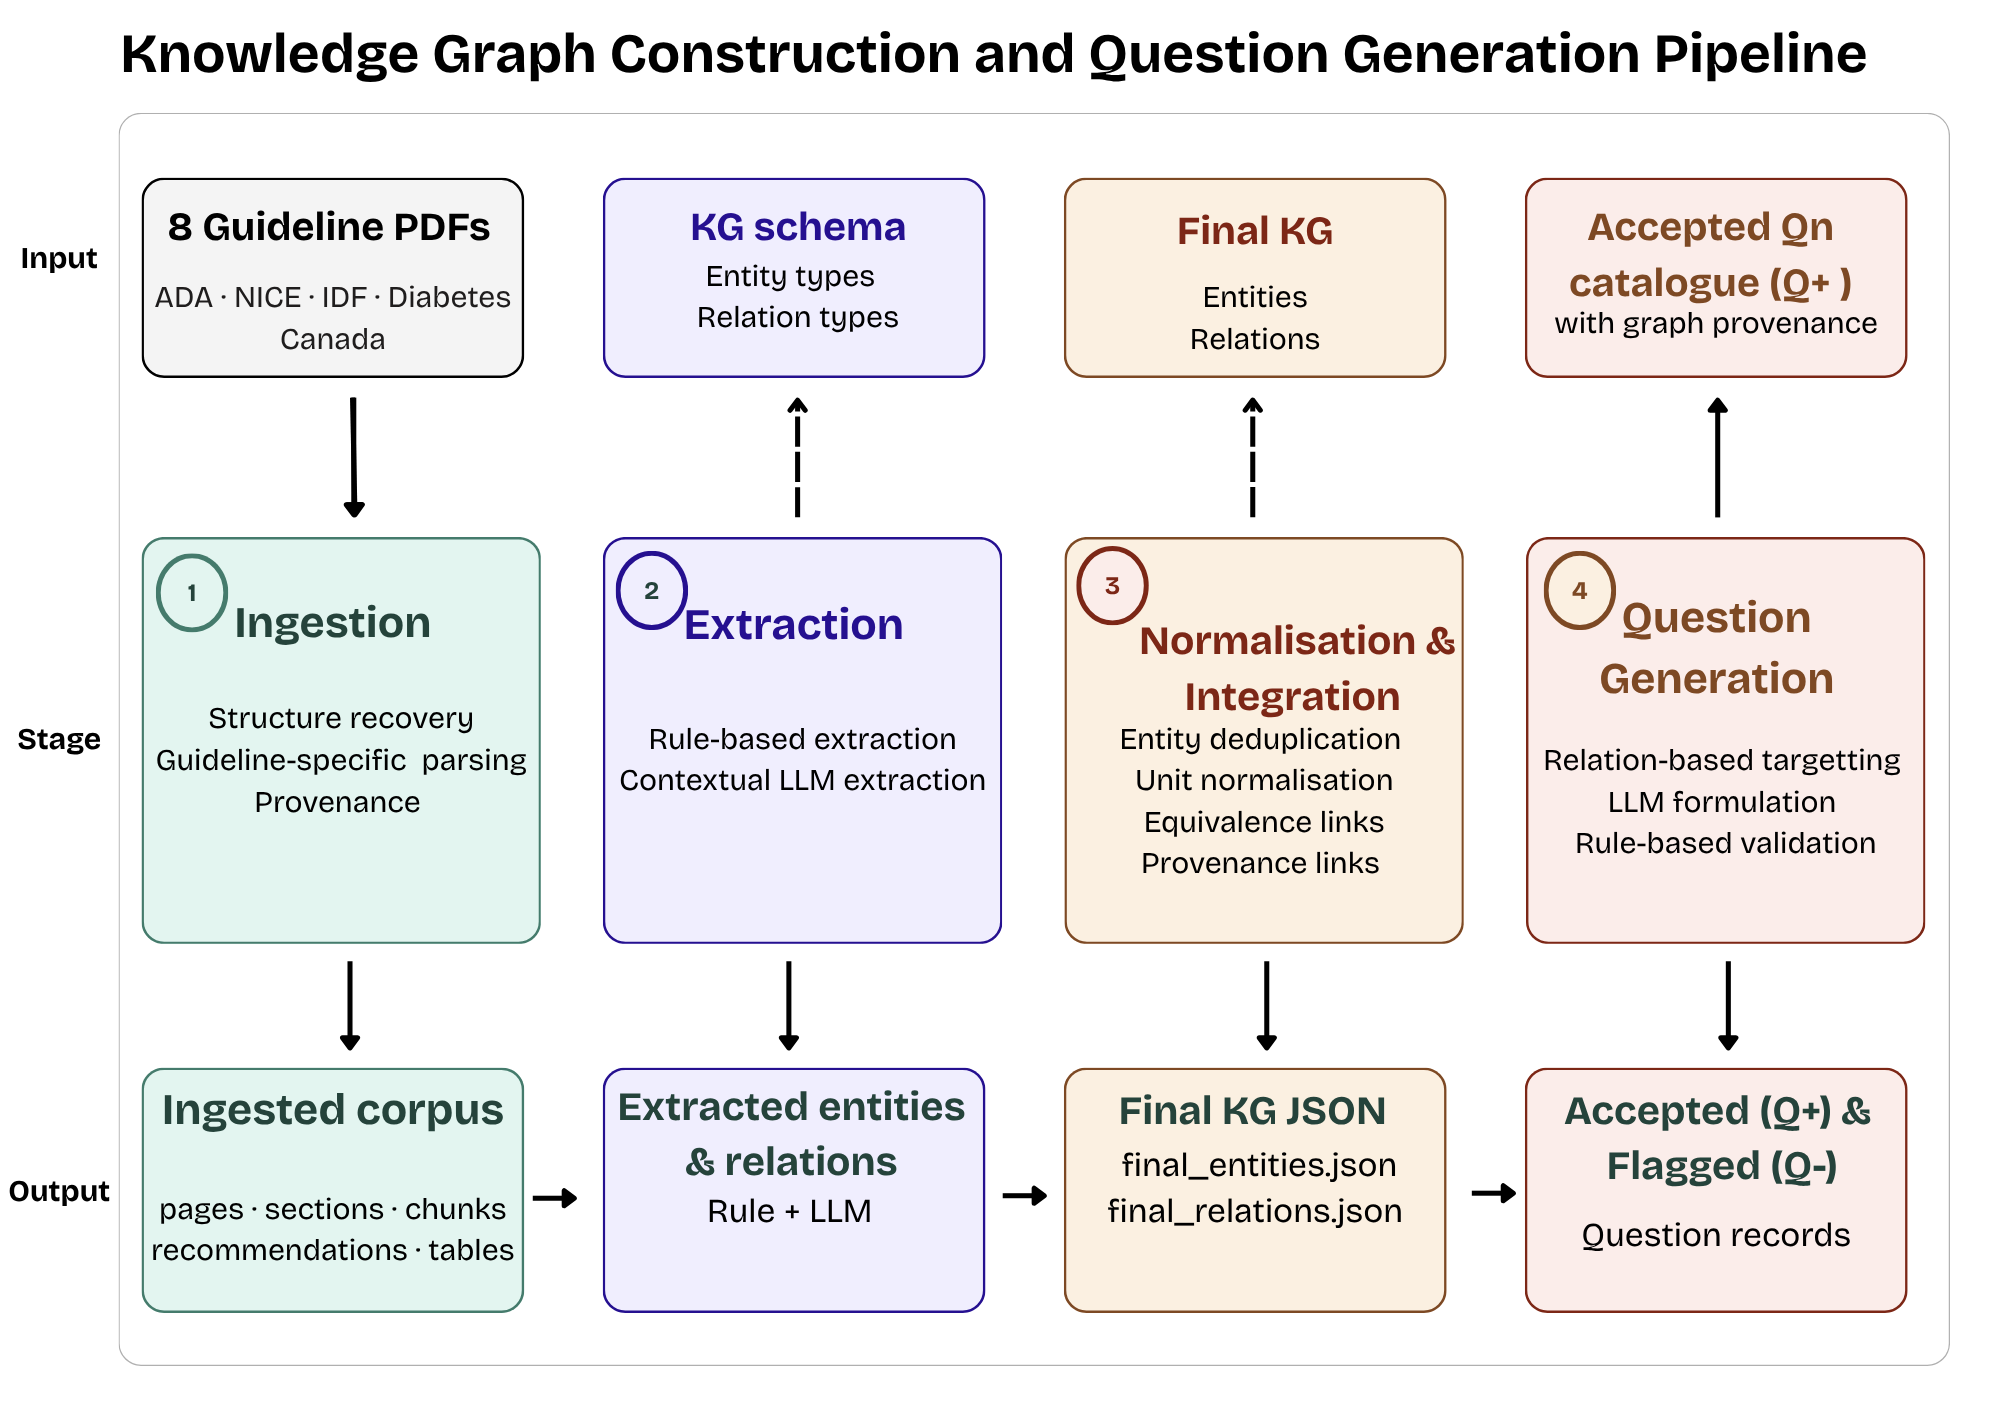
\includegraphics[width=\textwidth]{inc/figures/pipeline.png}
    \caption{Four-stage knowledge graph construction pipeline.}
    \label{fig:pipeline}
\end{figure}

Figure~\ref{fig:pipeline} shows the pipeline end to end. Guideline documents go into ingestion, which produces a structured representation of each document's content. Extraction reads that representation and produces two sets of typed entity and relation records, one from the rule-based layer and one from the language-model layer. Normalisation merges those two sets into one graph. Records referring to the same real-world entity are deduplicated into a single node, and numeric thresholds are converted to a common unit so equivalence edges can be detected. Question generation then walks the finished graph, selects eligible edges as anchors, and produces a validated set of clinical questions retaining the provenance available on their source graph relations

\section{Corpus Design}
\label{sec:corpus}

Building a Knowledge Graph that supports cross-guideline comparison requires a corpus that covers one clinical topic but varies in how that topic is presented. Using documents from a single organisation would produce a clean but narrow graph and defeat the purpose of cross-guideline comparison, so the corpus is selected against four criteria.

\paragraph{Geographic and systemic diversity}
Guidelines from different healthcare systems reflect different regulatory environments and patient populations. Using organisations from more than one country introduces variation in
guideline recommendations and healthcare-system context rather than only
the conventions of one national system.

\paragraph{Clinical coverage}
The selected guideline families need enough overlapping clinical content
for cross-guideline comparison to be possible. For this work, the common
coverage consists of diagnosis and classification, screening, glycaemic
targets, pharmacological management, and monitoring
\cite{ADA2026,NICE_T2_2026,IDF2025,CanadaDiabetes_Ch3}. A document covering
a narrower sub-topic can still be included where it contributes a
comparison point on one of these shared areas.

\paragraph{Format diversity}
Testing the pipeline against documents that all share one layout cannot show whether the pipeline generalises. The corpus requires documents that differ in how recommendations are laid out and in whether they use tables at all, so that ingestion and extraction face varied structure and not one convenient case.

\paragraph{Recommendation specificity}
Documents need to contain recommendations naming a specific drug, intervention, or measurement threshold, not high-level policy statements with nothing concrete to extract.

 The concrete outcome of applying these four criteria, i.e. which documents, how many pages, how many recommendations, is reported in Chapter~\ref{chap:evaluation}.

\subsection{Structural Heterogeneity as a Design Challenge}
\label{sec:heterogeneity}

Guideline documents from different organisations are not structurally uniform, and this shapes the design of every stage of the pipeline. Three dimensions of variation are particularly relevant to the pipeline.

\subsubsection{Recommendation format}

Some guidelines present recommendations as numbered, graded statements
that can be located by structural pattern. NICE's Type~2 diabetes
guideline uses this format throughout~\cite{NICE_T2_2026}:

\begin{quote}
\noindent
\textbf{1.13.1}\quad
\begin{minipage}[t]{0.82\linewidth}
For adults with type 2 diabetes and no relevant comorbidity, offer
modified-release metformin and an SGLT-2 inhibitor.
\hfill\textnormal{[2026]}
\end{minipage}
\end{quote}

The recommendation number, the imperative verb, and the update marker are
typographically consistent across the document and can be identified by
structural pattern matching. Metformin and SGLT-2 inhibitors are examples
of the \textsc{Drug} entities described in
Section~\ref{sec:node-types}.

The ADA Standards of Care also use numbered
recommendations, but place them within a multi-column layout alongside
commentary and cross-references~\cite{ADA2026}. For example:

\begin{quote}
\noindent
\textbf{9.21}\quad
\begin{minipage}[t]{0.82\linewidth}
In adults with type 2 diabetes without severe hyperglycemia or
hyperglycemic crisis, GLP-1-based therapy is preferred to insulin for
initial or add-on glucose-lowering therapy.
\hfill\textbf{A}
\end{minipage}
\end{quote}

Although both formats use numbered recommendations, their surrounding
document structure differs. The NICE recommendation can be located using
its consistent numbering and statement structure, whereas the ADA
recommendation must be identified within a three-column layout containing
additional commentary and cross-references. This difference affects how
the ingestion stage locates and extracts recommendation text.

\subsubsection{Tabular content}

Some guideline documents present diagnostic criteria in structured tables
rather than in numbered statements. This creates a different problem from
the numbering-versus-prose distinction above. The issue is not identifying
where a recommendation starts and ends, but reconstructing the row-and-column
structure before extraction can take place. The IDF and ADA documents present
some diagnostic criteria in this form. For example, ADA Table~2.1 includes
the following criteria~\cite{ADA2026}:

\begin{quote}
\textnormal{\textbf{Table 2.1: Criteria for the diagnosis of diabetes in
nonpregnant individuals}}\\[4pt]

FPG (fasting plasma glucose) $\geq 126$~mg/dL
($\geq 7.0$~mmol/L). Fasting is defined as no caloric intake for at least
8~h.\\[2pt]

\textit{OR}\\[2pt]

2-h PG (plasma glucose measured two hours into an OGTT, an oral glucose
tolerance test) $\geq 200$~mg/dL ($\geq 11.1$~mmol/L).
\end{quote}

When a naive text-stream extractor processes this page without spatial
reconstruction, the table structure collapses into a sequence of fragments
with no reliable row or cell boundaries. A simplified example of the
resulting text stream is shown below.

\begin{lstlisting}[
    language={},
    caption={Text-stream output from ADA Table 2.1 before spatial reconstruction.}
]
Table 2.1 Criteria for the diagnosis FPG 126 mg/dL 7.0 mmol/L
Fasting defined no caloric intake 8 h 2-h PG 200 mg/dL
11.1 mmol/L OGTT Random plasma glucose 200 mg/dL
\end{lstlisting}

Pattern matching for an expression such as
\texttt{FPG $\geq$ 126 mg/dL} fails on this output because the table
structure has collapsed and the comparison operators are not preserved in
the extracted text. The association between each metric and its corresponding
threshold can therefore no longer be recovered reliably from the text stream
alone. Spatial reconstruction of the row-and-column structure is required
before rule-based extraction of numerical thresholds from such pages.

The same extraction procedure cannot be assumed to apply to every guideline.
NICE NG17, for example, expresses comparable target information in prose
rather than in a table. Recommendation~1.6.6 states that adults with Type~1
diabetes should aim for an HbA1c level of 48~mmol/mol (6.5\%) or lower
\cite[recommendation 1.6.6]{NICE_T1_2022}. HbA1c (glycated haemoglobin) is
reported here in IFCC units (mmol/mol), which are discussed further below.
The ingestion pipeline therefore cannot assume that any single content
modality will be present across all guideline families.

\subsubsection{Measurement unit conventions}
Different organisations report the same class of measurement in different units. Plasma glucose values appear in mg/dL in the ADA document \cite{ADA2026} and in mmol/L in the NICE, IDF, and Diabetes Canada documents \cite{NICE_T2_2026,IDF2025,CanadaDiabetes_Ch3}. Glycated haemoglobin (HbA1c) appears as a percentage in some documents and in IFCC (International Federation of Clinical Chemistry) units (mmol/mol) in others; the standard method for relating the two scales is given by \cite{hoelzel2004}. Comparing numerical values across guidelines only works after unit normalisation, and only between values of the same kind. Cross-guideline comparison is restricted to targets that share the same
metric, operator, and normalised numerical value. The limitations of this
criterion are discussed in Chapter~\ref{chap:evaluation}.

These three dimensions of variation appear across all four guideline families in the corpus, and handling them without excluding a guideline family is a design requirement for the document-structuring and extraction stages described next.

Each of these three problems has been addressed individually in the
document-processing literature. PDF text extraction is a recognised difficulty
for scientific documents \cite{bast2017,ramakrishnan2012}, and tools such as
Docling combine layout analysis with table structure recognition
\cite{auer2024}. Table reconstruction has been studied for scientific articles
and document images \cite{zhong2020,schreiber2017}. Unit normalisation is
needed because clinical measurements are reported on different scales, for
example HbA1c in NGSP percent versus IFCC mmol/mol, which are related by a
linear regression \cite{hoelzel2004}. Here all three are handled within one
pipeline operating across four guideline families at once, without treating any
single family as the default case. The systems surveyed in
Section~\ref{sec:bg-related} address these problems individually, not in
combination.

\section{Structuring Guideline Documents for Extraction}
\label{sec:ingestion}

Clinical guideline documents are written for people, not software. Whatever format they arrive in, the actual clinical content is buried in a mix of typographic conventions, layout hierarchy, prose, numbered lists, and embedded tables, and none of that carries explicit markup a program can rely on. This is not really a PDF problem specifically. Human-oriented documents do not necessarily expose the semantic and structural information required by the downstream pipeline in a machine-readable form. Structuring the documents has three requirements. Each piece of content
needs a type, its position in the document structure needs to be retained,
and anything extracted from it later must remain traceable to the source.
The content model below represents these requirements explicitly.

\subsection{The Document Content Model}
\label{sec:content-model}

Ingestion works against a fixed content model. A guideline document $d \in \mathcal{D}$ is treated as an ordered sequence of content elements $e_1, e_2, \ldots, e_n$, and each element is a triple $e_i = (\tau_i,\ \text{text}_i,\ \pi_i)$, where $\text{text}_i$ is the extracted text, $\pi_i$ is a provenance record (defined below), and $\tau_i$ is drawn from a content-type set $\mathcal{T}_C$. $\mathcal{T}_C$ enumerates the structural units a document domain 
distinguishes, and in general it needs to separate free-form narrative 
content from any self-contained, explicitly delimited unit the document 
type uses. The distinction is structural, not semantic. A delimited unit has 
identifiable boundaries and usually a label the document itself 
supplies, so it can be located reliably and its identifier kept for 
provenance. Narrative text has neither. What $\mathcal{T}_C$ actually contains is a domain-specific configuration, not a fixed part of the model. For this corpus,
$$\mathcal{T}_C = \{\textsc{Prose},\ \textsc{Recommendation},\ \textsc{Table},\ \textsc{Section}\}$$
Chapter~\ref{chap:evaluation} describes how these four types were derived from the four diabetes guideline documents and gives the extraction rule used for each; a different document domain would likely need a different $\mathcal{T}_C$.

Each element's provenance has two levels. At the element level:
$$\pi_i^{\text{elem}} = (id_i,\ \text{sec\_id}_i,\ \text{sec\_title}_i,\ p_i^{\text{start}},\ p_i^{\text{end}})$$
$id_i$ is a unique element ID so anything extracted later can be traced back to it; $\text{sec\_id}_i$ groups elements by section for entity typing; $\text{sec\_title}_i$ is the actual heading text, which extraction uses to infer relation type; and $p_i^{\text{start}}, p_i^{\text{end}}$ are start and end page numbers, kept because any extracted claim needs to be checkable against the source page it came from. Elements of a self-contained, explicitly delimited type may carry an additional label field where the document itself provides one (e.g. a recommendation number), absent for other types. At the document level, a shared record resolves from $id_i$:
$$\pi_i^{\text{doc}} = (d_{\text{id}},\ \text{org},\ \text{geo},\ \text{source\_file})$$
covering the document ID, issuing organisation, healthcare system, and source filename.

Ingestion itself is a function $\varphi: \mathcal{D} \rightarrow 2^{\mathcal{E}}$, and it has to satisfy three things regardless of domain. \textit{Totality}: it produces output for every document, no document is allowed to come out empty just because, say, it lacks one particular content type. \textit{Type coverage}: across the whole corpus, every content type in $\mathcal{T}_C$ actually shows up at least once, so the ingestion logic cannot quietly collapse into handling only one modality. \textit{Provenance completeness}: every element that comes out has a fully populated $\pi_i$, so it can be traced back to a source location. Chapter~\ref{chap:evaluation} shows a concrete element produced by $\varphi$ for this corpus and how these three properties were verified against it.

\subsection{Structural Challenges in Ingestion}
\label{sec:ingestion-challenges}

PDF extraction is known to introduce artefacts like broken ligatures, lost word boundaries, and collapsed table columns \cite{bast2017,auer2024}. These are implementation-level engineering problems rather than conceptual ones, but the general requirement they impose on ingestion belongs here: the ingestion stage must detect and repair publisher-specific encoding artefacts before passing text downstream, since a corrupted token boundary breaks any pattern match or rule that assumes intact words. Two such challenges showed up often enough in this corpus to need dedicated handling; Chapter~\ref{chap:evaluation} gives the concrete encoding artefact encountered and the publisher-specific repair it required.

The first is extraction fidelity, i.e. documents from different publishers coming out of extraction looking very different internally, in ways that were not spread evenly across the corpus but tied to specific publishers' pipelines. A fix for this kind of artefact has to be written per publisher; one generic normalisation pass does not generalise across document families.

The second challenge is knowing where a recommendation actually ends. Even where the text extracts cleanly, grading scales, evidence summaries, and qualifying clauses sit typographically right next to the recommendation itself, and the boundary between "this is the recommendation" and "this is commentary about it" is not consistent across document families. No single rule covered all four families, so this was configured separately for each.

The complete set of typed, provenance-annotated elements from $\varphi$ is the only input the extraction stage (Section~\ref{sec:extraction}) receives --- no raw document text passes through beyond this point.

\section{Knowledge Graph Schema}
\label{sec:schema}

What the schema allows as a node or an edge determines what the graph can eventually be queried for. This section works through that schema in order: the formal graph model, then the node types, then the relation types, and finally why these particular types were chosen over the alternatives that were considered and dropped.

\subsection{Knowledge Graph Model}
\label{sec:graph-model}

The model used here is the labelled property graph, where nodes and edges are typed and can carry key-value properties \cite{hogan2021,hartig2014}. Formally, the graph is
\begin{equation}
G = (V,\ E,\ \mathcal{T}_V,\ \mathcal{T}_E,\ \phi,\ \psi,\ \lambda)
\label{eq:kg}
\end{equation}
where $\mathcal{T}_V$ is the node type set (Section~\ref{sec:node-types}) and $\mathcal{T}_E$ is the relation type set (Section~\ref{sec:relation-types}), defined before the rest of the tuple since both are used in what follows. $V$ is the set of nodes, and $E \subseteq V \times \mathcal{T}_E \times V$ is the set of directed typed edges, each edge $e = (v_i, r, v_j)$ connecting a source node to a destination node via a relation type $r \in \mathcal{T}_E$. $\phi: V \rightarrow \mathcal{T}_V$ assigns every node exactly one type, and $\psi: E \rightarrow \mathcal{T}_E$ assigns every edge exactly one relation type. $\lambda: V \cup E \rightarrow 2^{\mathcal{P}}$ maps nodes and edges to key-value properties; this is where clinical attributes and provenance metadata are stored.

Two things about the underlying requirements pushed this toward a property graph over RDF. In general, different entity types need different attribute sets: in this corpus, for example, a \textsc{GlycaemicTarget} node needs a metric name, an operator, a value, and a unit, while a \textsc{Drug} node needs none of those. A property graph handles this directly through $\lambda$. RDF would need a separate triple per attribute, splitting one clinical fact across several statements \cite{barrasa2023}. Provenance was the second factor. Clinical relationships need to remain
traceable to their source context, so provenance must be representable on
edges as well as on nodes. Property graphs support edge properties directly. RDF needs named-graph reification or the singleton property pattern to attach metadata to a statement, which adds structural overhead without a corresponding benefit for this use case.

The corpus $\mathcal{D} = \{d_1, d_2, \ldots, d_n\}$ is the only factual source for $G$. Building $G$ means applying the extraction function $\xi$ (Section~\ref{sec:extraction}) to the output of $\varphi$, then applying the normalisation function $\eta$ (Section~\ref{sec:normalisation}) to merge the result into a deduplicated instance of $G$.

\subsection{Node Types and Their Roles}
\label{sec:node-types}

The node type set is:
\begin{align*}
\mathcal{T}_V = \{\textsc{Organisation},\ \textsc{Guideline},\ 
\textsc{Condition},\ \textsc{Drug},\ \textsc{ClinicalCondition},\ \\
\textsc{Intervention},\ \textsc{Population},\ \textsc{GlycaemicTarget},\
\textsc{Recommendation},\ \\ \textsc{MonitoringProtocol},\ 
\textsc{Table},\ \textsc{Test},\ \\ \textsc{TreatmentRecommendation}\}
\end{align*}

These thirteen types came from inspecting the four guideline families in the corpus \cite{ADA2026,NICE_T2_2026,IDF2025,CanadaDiabetes_Ch3}, not from an existing medical ontology, and no claim is made that the same thirteen types would work in another clinical domain. An initial list was drawn from the recurring subjects of the recommendation statements, then went through two rounds of manual review. Types that could not be reliably populated from the corpus were dropped, and types that were quietly conflating two different subjects were split apart. The thirteen types split across three categories: global types,
organisation-scoped types, and structural types that sit outside both
scoping levels.

\subsubsection{Global node types}
A drug is the same drug no matter which guideline mentions it, and a clinical condition is the same condition no matter which body defines it. These concepts are represented as global nodes, independent of any one guideline, and that independence is what makes cross-guideline comparison possible in the first place. A single global \textsc{Drug} node can participate in \textsc{first\_line\_for} relations originating from several guidelines, allowing recommendations about the same drug to be compared directly. The global types are \textsc{Drug}, \textsc{Condition}, \textsc{ClinicalCondition}, \textsc{Intervention}, and \textsc{Test}.

\subsubsection{Organisation-scoped node types}
A glycaemic target value stated in one guideline is not automatically the same statement as a numerically similar value in another. Each is issued by a specific organisation, for a specific patient population, and merging the two on numerical similarity alone would erase that distinction. Organisation-scoped nodes keep each guideline's own position separate by carrying the issuing body as a required property. The organisation-scoped types are
\textsc{GlycaemicTarget}, \textsc{Recommendation},
\textsc{TreatmentRecommendation}, \textsc{MonitoringProtocol},
and \textsc{Table}.

\subsubsection{Structural node types}
Three types are structural, not clinical. \textsc{Organisation} nodes represent the guideline-issuing bodies and sit at the root of the provenance hierarchy. \textsc{Guideline} nodes represent individual published documents and connect to their issuing organisation by a \textsc{publishes} edge. Where a direct structural relation exists, such as \textsc{has\_recommendation} or \textsc{contains\_table}, the extracted node is linked directly to its source guideline; other organisation-scoped nodes retain guideline-level provenance through organisation and source metadata rather than a direct edge. \textsc{Population} nodes represent patient subgroups, letting the graph
distinguish a recommendation for all adults with Type~2 diabetes from
one aimed at a more narrowly defined subgroup. The corpus contains many
such subgroups stated at different levels of specificity, for example
distinctions by age, by pregnancy status, or by a named comorbidity.
Population is treated as structural, not global, because these
subgroup descriptions are worded differently across organisations and
in some cases across recommendations from the same organisation; in
the corpus, a subgroup only carries meaning in relation to the specific
recommendation and guideline that names it.
A small example shows why Population is kept structural. The
population descriptions are extracted contextually rather than by
fixed pattern. ADA recommendations reference an older-adult subgroup using several
different phrasings across different recommendations, including
"older adults with type~2 diabetes," "older adults," and
"individuals aged~70~years and older." These are not treated as one
canonical Population node the way \textsc{Drug} mentions of metformin
are, because merging them would erase which specific recommendation
each phrasing came from, and because the boundary of "older" is not
stated consistently even within a single guideline.


\subsection{Relation Types and Their Semantics}
\label{sec:relation-types}

The relation type set is:
\begin{align*}
\mathcal{T}_E = \{\ &\textsc{publishes},\ \textsc{has\_recommendation},\ \textsc{contains\_table},\ \\
&\textsc{first\_line\_for},\ \textsc{second\_line\_for},\ \textsc{recommended\_for},\ \\
&\textsc{contraindicated\_in},\ \textsc{manages},\ \textsc{used\_with},\ \\
&\textsc{associated\_with},\ \textsc{has\_target},\ \textsc{specifies\_target},\ \\
&\textsc{measured\_by},\ \textsc{requires\_monitoring},\ \textsc{has\_protocol},\ \\
&\textsc{describes\_protocol},\ \textsc{mentioned\_in},\ \textsc{equivalent\_to}\ \}
\end{align*}

These eighteen relation types are derived from recurring relationships
in the corpus together with the structural and provenance requirements
of the graph. Clinical relation types reflect relationships stated in
the guideline content, while structural and provenance relations encode
document organisation and traceability. The
\textsc{equivalent\_to} relation is different again: it is created
during normalisation rather than extracted from text.

Relation types are retained only where they represent a distinction
needed by the graph and could be populated reliably from the corpus. For
example, \textsc{first\_line\_for} and \textsc{second\_line\_for} remain
separate because merging them into \textsc{recommended\_for} would remove
the treatment-sequence distinction expressed in the source guidelines.

\subsubsection{Pharmacological relations}
These relations record treatment decisions. The guidelines give a drug's position in a treatment sequence, not just an association with a condition, so the schema needs to represent sequence. "First-line" and "second-line" refer to the order treatments are tried in, not to drug quality.

\textsc{first\_line\_for} and \textsc{second\_line\_for} are kept as separate types because the guidelines themselves use the terms "first-line" and "second-line" directly in the recommendation text \cite{NICE_T2_2026}. \textsc{recommended\_for} is a weaker type for cases where a guideline endorses a treatment without placing it in that hierarchy, which shows up often in guidelines whose tiered-care structure does not map cleanly onto first- or second-line. \textsc{contraindicated\_in} records that a drug should not be used in a given context; leaving it out would have meant the graph could only represent positive recommendations. \textsc{manages} links an intervention to a condition without naming a treatment-sequence position, which is common for non-pharmacological interventions such as lifestyle changes. \textsc{used\_with} records two agents named together in one recommendation. NICE recommendation 1.13.1 \cite{NICE_T2_2026} names modified-release metformin and an SGLT-2 inhibitor in a single statement, and representing that as two separate \textsc{first\_line\_for} edges would lose the fact that the source names them together. \textsc{associated\_with} is used for a weaker descriptive relation where
the source links a clinical concept to another concept without stating a
treatment recommendation, contraindication, or management relation.

Three relation types were considered here and dropped. \textsc{preferred\_over} would assert a direct comparative ranking between two drugs. In the four guidelines examined, preference between drugs was stated inconsistently and with population-specific qualifications attached, which made reliable extraction impractical; the same preference order can already be inferred by comparing the \textsc{first\_line\_for} and \textsc{second\_line\_for} edges on a shared condition node, so a dedicated relation was not needed. \textsc{dosage\_of} was dropped because dosage statements in the corpus are heavily conditioned on population, timing, renal function, age, and comorbidity, and a single binary edge cannot represent that. \textsc{causes}, for adverse effects, was dropped because adverse-effect statements are written in prose too variable to decompose reliably into clean drug-effect pairs.

\subsubsection{Monitoring and measurement relations}
A condition may be linked to a glycaemic threshold through
\textsc{has\_target}. This relation is created only when the surrounding
source context identifies the diabetes type unambiguously. If the context
does not distinguish Type~1 from Type~2 diabetes, the
\textsc{GlycaemicTarget} remains in the graph with its provenance but no
disease-specific \textsc{has\_target} relation is added. The target may
be linked to the relevant test through \textsc{measured\_by}, and a drug or condition may be linked to a monitoring protocol through
\textsc{requires\_monitoring}.

For example, when a passage explicitly identifies Type~1 diabetes and
states a numerical glycaemic target, the resulting target can be linked
to the global \textsc{Type 1 Diabetes} condition node. A numerical target
that does not establish whether the surrounding statement concerns
Type~1 or Type~2 diabetes is retained without such a condition-specific
edge. This avoids assigning a disease scope that is not supported by the
local source context.

\textsc{specifies\_target} links a \textsc{Recommendation} or \textsc{Table} node to the \textsc{GlycaemicTarget} it states explicitly. This edge is created only when the numerical target is extracted from an element with a known identity in the graph; targets extracted from general prose chunks, which have no such element to point back to, receive no \textsc{specifies\_target} edge. \textsc{has\_protocol} links a clinical concept to a
\textsc{MonitoringProtocol} associated with its monitoring requirements.
\textsc{describes\_protocol} links a source element, such as a
recommendation or table, to the \textsc{MonitoringProtocol} whose
procedural content it describes.

This chain exists because comparing thresholds across organisations is one of the central objectives of the graph, and that comparison needs a structured place to point to. \textsc{has\_target} points to a formally defined \textsc{GlycaemicTarget} node, which is what gets normalised and later carries an \textsc{equivalent\_to} edge. \textsc{requires\_monitoring} is kept separate from \textsc{has\_target} because a monitoring protocol is procedural, not numerical; it specifies what to check and how often, not a threshold value. \textsc{measured\_by} connects a  \textsc{GlycaemicTarget} to the diagnostic test used to assess it, and scopes the unit-normalisation problem: two targets for the same condition, measured by the same test but expressed in different units, become candidates for an \textsc{equivalent\_to} edge once normalised. A \textsc{frequency\_of} relation was considered but dropped, since monitoring-frequency statements in the corpus sit inside conditional clauses that would need a much richer event model to represent properly.

\subsubsection{Cross-guideline and provenance relations}
These relations give the graph its multi-guideline and provenance structure. They connect organisations, documents, extracted content, and cross-guideline comparison results.

\textsc{publishes}, \textsc{has\_recommendation}, and
\textsc{contains\_table} provide the main document-level provenance
links. An \textsc{Organisation} connects to its \textsc{Guideline}
nodes through \textsc{publishes}. A \textsc{Guideline} connects to its
\textsc{Recommendation} nodes through \\ \textsc{has\_recommendation} and
to its \textsc{Table} nodes through \textsc{contains\_table}. Together,
these relations preserve the connection between document content and
the organisation that issued the guideline.

\textsc{mentioned\_in} is a provenance relation linking a global entity to the guideline in which it occurs. These links are created during normalisation from the entity's recorded guideline mentions and are retained independently of any more specific clinical relations involving the same entity.

\textsc{equivalent\_to} is not extracted from text. It is created during
normalisation when two \textsc{GlycaemicTarget} nodes from different
guidelines share the same metric, operator, and normalised value after
unit conversion. It provides the mechanism used in this work to represent
cross-guideline agreement on a numerical threshold.

Two further types were considered and dropped from this group. \textsc{supersedes}, for one recommendation replacing an older one from the same organisation, would need a model of guideline update cycles over time, which is out of scope for a corpus frozen at a single point in time. \textsc{contradicts} was also considered, but disagreement between
organisations was not represented as an explicit relation in the source
documents. Differences can instead be identified by comparing
\textsc{first\_line\_for} or \textsc{has\_target} edges associated with
the same condition. Whether such a difference constitutes a clinical
contradiction is not determined by the graph.

\subsection{Schema Design Rationale}
\label{sec:schema-rationale}

The schema balances two requirements that pull in opposite directions.
It needs enough types to preserve distinctions that matter in the source
guidelines, but every additional type also has to be populated reliably.
For example, collapsing \textsc{first\_line\_for} and
\textsc{second\_line\_for} into \textsc{recommended\_for} would make
extraction simpler, but it would remove treatment order from the graph.
At the other extreme, a relation such as \textsc{dosage\_of} looks useful
in principle but would need more structure than a single edge can carry.
No systematic optimisation over alternative schema sizes is performed.
The retained types are those for which the distinction is useful to the
queries supported by the graph and for which the corpus provides enough
structure to populate the type consistently. The rejected relation types
and their individual reasons are discussed with the corresponding
relation groups above.

Figure~\ref{fig:schema} illustrates the node-scoping structure and representative relations in the Knowledge Graph. The node columns show representative node types from the global, structural, and organisation-scoped categories. The arrows show representative examples from the three relation groups: pharmacological, monitoring and measurement, and cross-guideline and provenance. The complete set of eighteen relation types is defined in $\mathcal{T}_E$ above.

\begin{figure}[!ht]
    \centering
    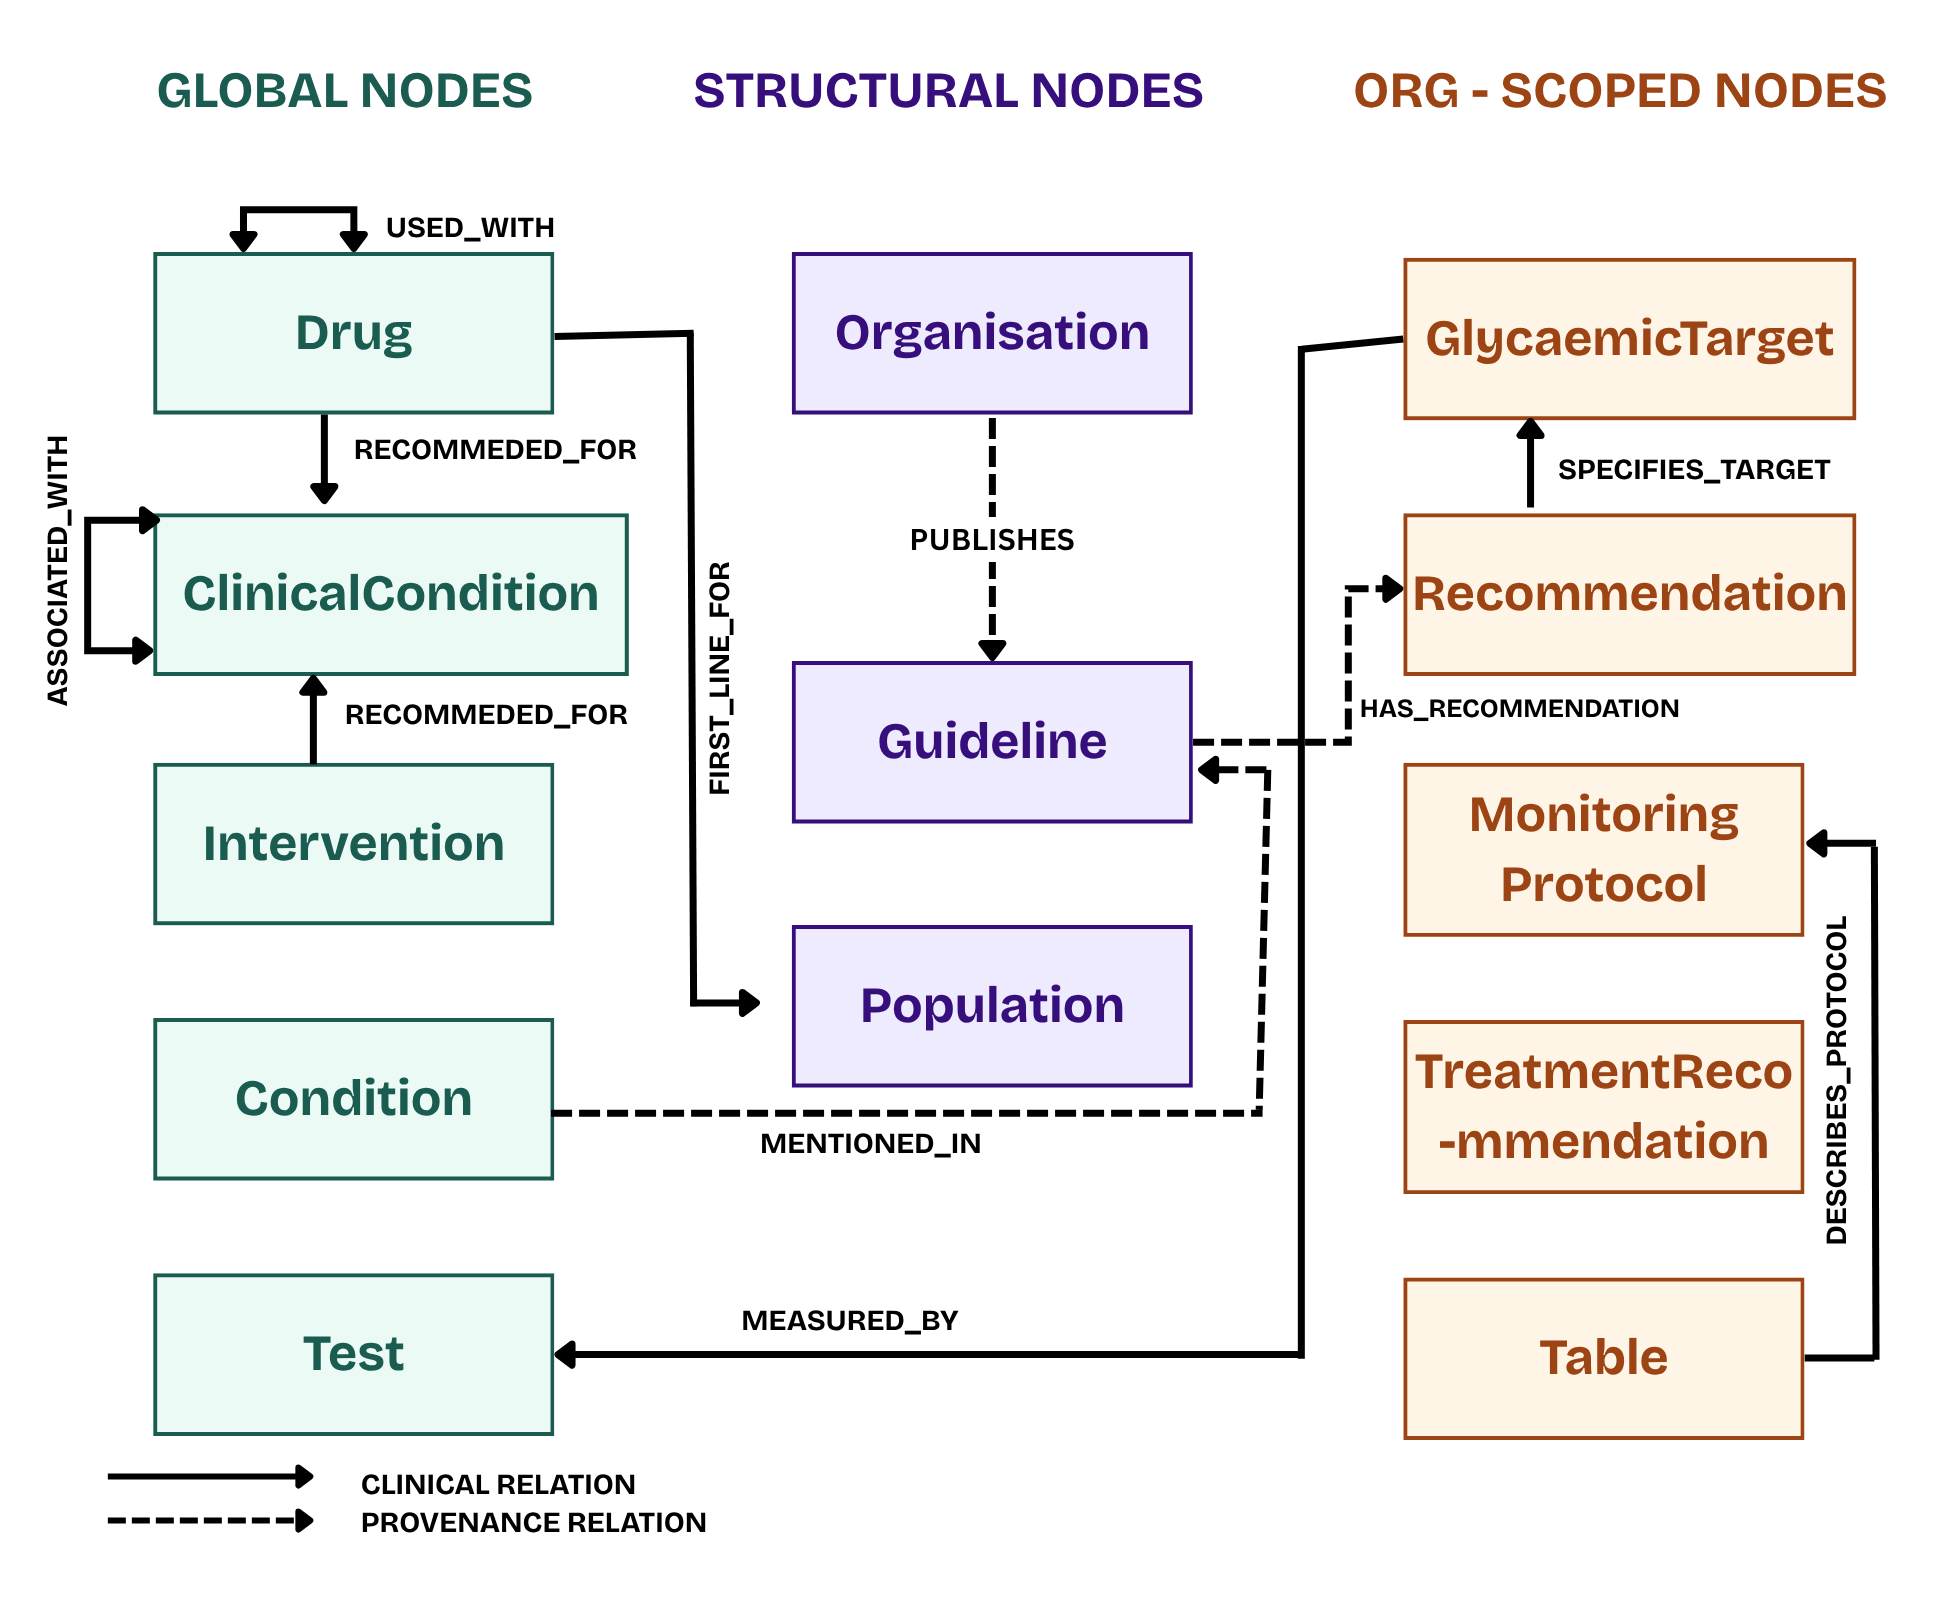
\includegraphics[width=\textwidth]{inc/figures/kg_schema.png}
    \caption{Knowledge Graph Schema}
    \label{fig:schema}
\end{figure}

Global nodes are what let edges cross between guidelines at all; leaving them out would mean each guideline produces its own isolated subgraph. Organisation-scoped nodes prevent the opposite problem. Leaving them out would merge every guideline's specific position into one shared node per concept, erasing the variation that cross-guideline comparison is meant to surface.

\section{Entity and Relation Extraction}
\label{sec:extraction}

The extraction stage reads the structured records produced by $\varphi$ and identifies the clinical entities and relations that become nodes and edges in the graph. This is where content elements from $\mathcal{T}_C$ turn into typed graph elements drawn from $\mathcal{T}_V$ and $\mathcal{T}_E$, and it is where the main architectural decisions sit. Three matter most. Which entity types go to which extraction layer, how the language model is constrained, and how identity is kept consistent across documents.

Two difficulties were particularly important in this corpus. The first is terminological precision. Clinical guidelines use controlled vocabulary where small differences in wording carry large differences in meaning; in the corpus documents, a drug described as "recommended" is not the same as one described as "preferred", which is not the same again as one "considered as an option". An extraction method that treats these as equivalent produces a graph that misstates how strongly a guideline actually recommends something. The second is cross-document consistency: the same concept can be worded differently across guidelines, for example "type~2 diabetes" in one and "non-insulin-dependent diabetes mellitus" in another, so extraction has to produce identifiers that match across documents, not only within one. Named entity recognition and relation extraction as techniques are background covered in Chapter~\ref{chap:background} \cite{nasar2021,zhao2024}; what this chapter contributes is not the techniques themselves but the specific architecture through which they are applied to a multi-guideline clinical corpus.

\subsection*{The Extraction Function}

Extraction is usually split into entity recognition and relation extraction as separate steps \cite{nasar2021}; here both are combined into one function:
\begin{equation}
\xi: 2^{\mathcal{E}} \rightarrow \mathcal{V} \times \mathcal{R}
\label{eq:extraction}
\end{equation}
where $2^{\mathcal{E}}$ is the power set of element records produced by $\varphi$, $\mathcal{V}$ is the set of typed entity records, and $\mathcal{R}$ is the set of typed relation records. An entity record $v \in \mathcal{V}$ is a tuple
$$v = (\text{id}_v,\ \tau_v,\ \text{name}_v,\ \pi_v,\ m_v)$$
where $\tau_v \in \mathcal{T}_V$ is the entity type, $\text{name}_v \in \mathbb{S}$ is the canonical surface form, $\pi_v$ is the provenance inherited from the source element, and $m_v \in \{\textsc{Rule}, \textsc{LLM}\, \emptyset\}$ records which layer produced it. A relation record $r \in \mathcal{R}$ is
$$r = (\text{id}_r,\ \text{src}_r,\ \psi_r,\ \text{dst}_r,\ \pi_r,\ m_r)$$
where $\psi_r \in \mathcal{T}_E$ is the relation type, $\text{src}_r$ and $\text{dst}_r$ are entity identifiers, $\pi_r$ is provenance, and $m_r$ is the method label. This method label is what makes each layer's contribution checkable on its own during normalisation and later evaluation, instead of only as a combined result.

\subsection{Rule-Based Extraction}
\label{sec:rule-extraction}

Rule-based extraction applies pattern matching and structural heuristics directly to the element records to pull out a specific, limited set of entity and relation types. Rather than trying to extract everything, the rule layer only targets types that have a reliable structural or lexical signal in the guideline text.

A type is assigned to the rule layer when its instances have a predictable
syntactic or structural form that is sufficiently consistent in the
document families where that type occurs. Types that do not meet this
condition are assigned to the contextual extraction layer.

\paragraph{GlycaemicTarget entities}
A numerical target has a local structure that can be decomposed directly.
For example,
\[
\text{FPG} \geq 7.0~\text{mmol/L}
\]
contains the metric \texttt{FPG}, the operator $\geq$, the value
\texttt{7.0}, and the unit \texttt{mmol/L}. These four fields are captured
separately by the rule layer: a regular expression matches the metric
name and unit as fixed anchors, with the operator and numeric value
extracted as separate groups in between. The gap between the metric
name and the operator is allowed to contain up to 40 or 60 characters
of intervening text, depending on the metric, so the same pattern still
matches when a guideline states the target inside a longer sentence
rather than as a short standalone expression. A second instance
illustrates this with a different metric and unit,
\[
\text{HbA1c} \geq 48~\text{mmol/mol},
\]
extracted by a separate but structurally identical pattern. The
surrounding sentence may vary, but the target itself retains the same
four-field structure in both cases.

\paragraph{MonitoringProtocol entities}
come from two sources. Prose containing continuous glucose monitoring
or time-in-range terminology, matched by terms such as
\textit{time in range}, \textit{TIR}, and \textit{CGM}, produces one
\textsc{MonitoringProtocol} node per organisation. These mentions can
recur throughout a document, so creating a new node for every occurrence
would represent the same monitoring concept several times. Table captions
provide the second route. A caption containing monitoring-related terms
such as \textit{monitor}, \textit{screen}, \textit{follow-up}, or
\textit{frequency} produces a \textsc{MonitoringProtocol} associated
with that table. Both cases have an explicit lexical or structural signal
and are therefore handled by the rule layer without a language-model call.

\paragraph{TreatmentRecommendation entities}
are extracted from tables rather than from numbered
\textsc{Recommendation} elements. A table whose caption contains
treatment-related vocabulary such as \textit{treat}, \textit{therap},
\textit{pharmac}, \textit{drug}, \textit{medic}, or \textit{insulin}
produces a \textsc{TreatmentRecommendation} node. This is distinct from
a \textsc{Recommendation} node, whose boundary and recommendation number
come from the numbered guideline statements identified during document
structuring. The schema keeps the two types separate because they
represent two different source structures: one is an explicitly numbered
guideline statement and the other is a treatment summary identified from
a table.

\paragraph{Canonical anchor nodes}
\textsc{Condition} and \textsc{Test} do not follow the same extraction
route as the entity types above. A fixed list of five \textsc{Condition} nodes
(Type~1 Diabetes, Type~2 Diabetes, Prediabetes, Intermediate
Hyperglycaemia, and Gestational Diabetes) is created before extraction
begins rather than being extracted independently from each document. \textsc{Test} nodes are created when extraction encounters a named test,
such as HbA1c or CGM, but repeated occurrences of the same test name
resolve to the same global node. The identity problem is therefore different in the two cases. For
\textsc{Condition}, identity is fixed before extraction. For
\textsc{Test}, identity is resolved by exact name matching when a test
is encountered. Both types can subsequently be supplied to the LLM layer
as known entities, as described in Section~\ref{sec:llm-extraction}.

Rule-based extraction is interpretable and deterministic. Every entity traces
back to the pattern that produced it, and a false positive can be investigated
by examining or modifying that pattern, which is one reason rule-based systems
remain widely used in practice \cite{chiticariu2013}. Its limitation is
coverage. In the guidelines processed here, drug indications stated across several
clauses, contraindications buried in qualifying remarks, and
population-specific modifications inside conditional phrasing eluded reliable
pattern matching. This coverage gap motivates the LLM-based layer, since
language models can extract structured information from text with little
task-specific training data \cite{xu2024,caufield2024}.

\subsection{LLM-Based Extraction}
\label{sec:llm-extraction}

The contextual extraction layer identifies entities and relations that need contextual reading, where pattern matching alone won't work, and targets the entity types that are beyond what a rule can reliably reach. Both layers operate on the structured document records produced by $\varphi$, but the contextual layer additionally receives page-level facts already identified by the rule layer as grounding context. The two layers are therefore separated by target category rather than by independent execution.

\paragraph{The constrained generation context.}
The main risk in applying a language model to clinical text is hallucination \cite{huang2025}. An incorrect drug indication or a fabricated contraindication is a worse failure here than in most extraction tasks, so the design leans toward traceability and grounding over raw coverage. Prior work on schema-constrained prompting shows that giving a model an explicit output schema as a generation constraint reduces hallucination in knowledge-base population; the LLM layer here follows the same principle, operating under a constrained generation context
$$\mathcal{C} = (\mathcal{T}_V,\ \mathcal{T}_E,\ \mathcal{K})$$
where $\mathcal{T}_V$ and $\mathcal{T}_E$ are the allowed entity and relation types, and $\mathcal{K}$ is the page-level set of structured facts already identified by deterministic extraction. In the implementation, this context contains numerical targets and recommendation records associated with the current page. Page-level scope is used for $\mathcal{K}$ for two reasons. A chunk-level
scope is too narrow because a numerical target or recommendation identified
in one element on a page may provide relevant grounding for another element
on the same page. A document-level scope is too broad, since passing facts
from the entire guideline would add information unrelated to the passage
being processed. Page-level scope therefore preserves nearby grounding
information while keeping the context focused on the current page.

$\mathcal{C}$ is injected into the model's prompt as a prompt-level constraint. The system prompt lists the allowed entity and relation types directly and instructs the model to restrict its output to types already present in $\mathcal{T}_V$ and $\mathcal{T}_E$. This is an instruction rather than an enforced constraint. The API call guarantees only that the response parses as structured output. The parser does not reject records whose type falls outside the declared sets, so compliance rests on the model following the instruction. In the reported run, two relation records used undeclared relation types (researching and intervention). These records were excluded from the final graph during integration.

Together, these two constraints define what the model is asked to do. It classifies and structures content from the input passage, using surface forms and identities the rule layer and schema have already set. Nothing beyond the passage, the schema, and the page-level rule-derived context \(K\) is supplied to it. Whether the model also draws on its own parameters is not something the output can tell us.

\paragraph{LLM extraction targets.}
Four entity types go to the LLM layer because rule-based methods cannot reliably reach them. \textsc{Drug} entities appear throughout guideline prose in varying syntactic positions --- as the subject of a recommendation clause, the object of a contraindication statement, or a member of an enumerated drug class --- and picking them out needs the kind of contextual reading a language model does well. Metformin, for example, may appear as the treatment
being recommended, as part of a combination, or inside a statement that
qualifies when it should be used. Its syntactic position therefore does
not provide the stable cue available for a numerical target.
\textsc{Population} entities, describing the patient group a recommendation applies to, are often long noun phrases with several qualifying modifiers, which makes pattern matching unreliable. \textsc{ClinicalCondition} entities, covering comorbidities and complications that interact with diabetes management, are worded very differently across the four guideline families. \textsc{Intervention} entities, covering non-pharmacological approaches such as lifestyle change or surgery, use terminology that varies enough between organisations that a fixed dictionary lookup would not hold up.

For relations, the LLM layer targets ones that need reasoning across more than one sentence: \textsc{contraindicated\_in} relations stated across conditional clauses, \textsc{used\_with} relations implied by a description of combination therapy, and \textsc{manages} relations asserted through treatment narrative, not an explicit recommendation statement.

\paragraph{Separation and auditability.}
Figure~\ref{fig:extraction} makes one design decision explicit. The rule and contextual components are assigned disjoint entity categories rather than competing to extract the same types. Contextual extraction can use facts already identified by the rule layer as grounding information, but it does not act as a fallback that simply fills every gap left by the rules. Method labels retained on extracted records allow the contribution of each extraction route to be inspected separately.

\begin{figure}[!ht]
    \centering
    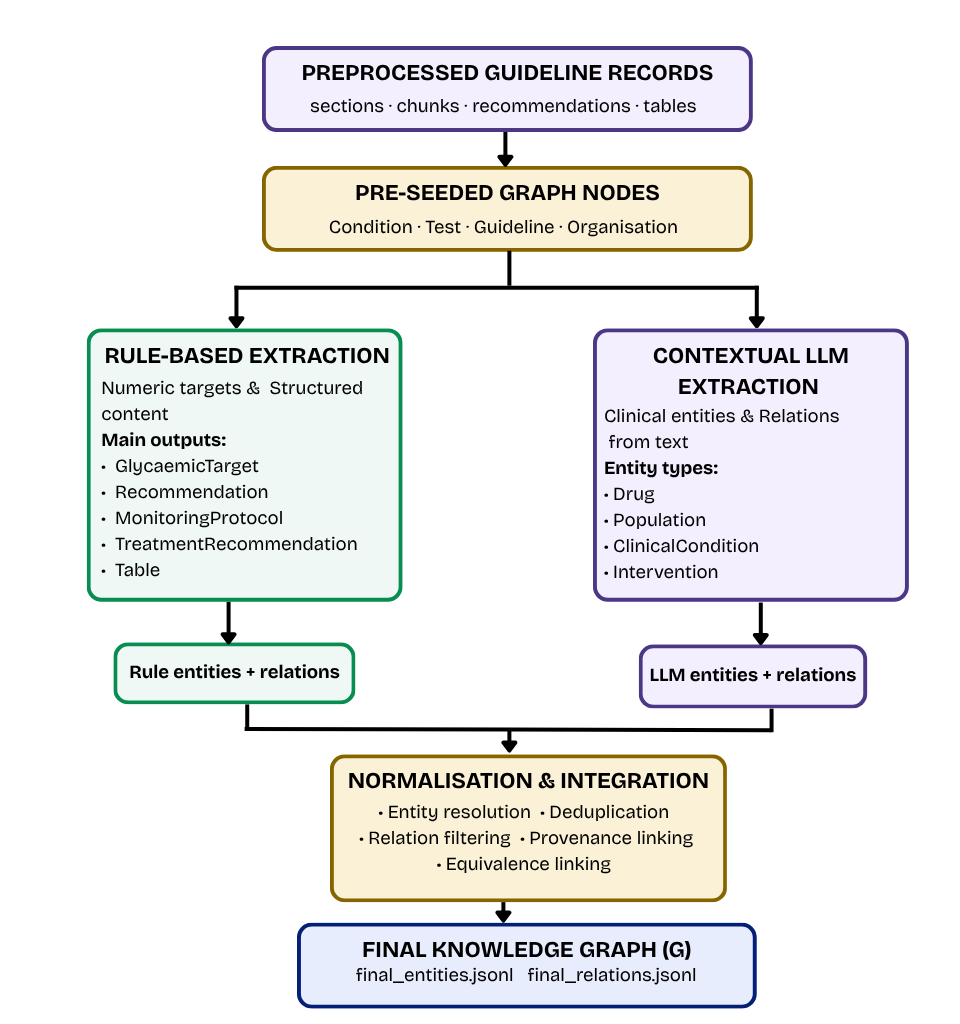
\includegraphics[width=\textwidth]{inc/figures/extraction_architecture.png}
    \caption{Layered extraction architecture}
    \label{fig:extraction}
\end{figure}

The output of both layers, the entity records in $\mathcal{V}$ and relation records in $\mathcal{R}$, passes to the normalisation stage, which resolves duplicates, converts units, and integrates both record sets into the finished graph $G$, described next in Section~\ref{sec:normalisation}.

\section{Normalisation and Graph Integration}
\label{sec:normalisation}

The normalisation stage takes the entity records $\mathcal{V}$ and relation records $\mathcal{R}$ produced by $\xi$ and integrates them into the unified graph $G$. It addresses three problems the extraction stage necessarily leaves unresolved --- entity duplication, terminological variation, and unit inconsistency. Entity deduplication is studied in the entity resolution and record linkage
literature \cite{getoor2012,christen2012,brizan2015}, and mapping biomedical
mentions to standard concepts is a long-standing task in clinical NLP, for
example for disease names \cite{singh2013}. Unit normalisation is needed here
because clinical measurements are reported on different scales across
guidelines \cite{hoelzel2004}. The contribution of this stage is applying both
steps within one multi-guideline pipeline.

The normalisation stage is formalised as a function
\begin{equation}
\eta: (\mathcal{V} \times \mathcal{R}) \rightarrow G
\label{eq:normalisation}
\end{equation}
where $G = (V, E, \mathcal{T}_V, \mathcal{T}_E, \phi, \psi, \lambda)$ is the graph defined in Section~\ref{sec:graph-model}. $\eta$ has to satisfy two properties. \textit{Provenance monotonicity}: merging two records never reduces the provenance carried by the result, since the provenance of the merged element is the union of everything that went into it.

\subsection{Entity Deduplication}
\label{sec:deduplication}

Both extraction layers can independently identify the same real-world entity from different passages of the same document, or from different documents entirely, producing more than one record for the same concept. Loading those duplicates into the graph without resolving them first would leave several near-identical nodes standing in for one entity, splitting relations that should converge on a single node across all of them and making cross-guideline queries incomplete.

Deduplication uses a type-specific equivalence relation $\sim_\tau$ over entity records. Two records $e_i, e_j$ of type $\tau$ count as duplicates exactly when $e_i \sim_\tau e_j$, and are then merged into one node whose provenance is the union of $\pi_{e_i}$ and $\pi_{e_j}$. This relation takes two different forms, depending on the structural properties of the type.

\paragraph{Name-bearing entity types.}
For types whose identity is a canonical name string --- \textsc{Drug}, \textsc{Condition}, \textsc{ClinicalCondition}, \textsc{Intervention}, and \textsc{Test} --- the equivalence relation is
$$e_i \sim_\tau e_j \iff \sigma(\text{name}(e_i)) = \sigma(\text{name}(e_j))$$
where $\sigma: \mathbb{S} \rightarrow \mathbb{S}$ normalises a surface form in three steps: it collapses whitespace and strips leading and trailing spaces, applies Unicode case folding, and then maps the result through a type-specific canonicalisation dictionary $\Delta_\tau: \mathbb{S} \rightarrow \mathbb{S}$ that resolves known surface-form variants to one canonical representative. In the implementation, separate alias mappings are used for different
name-bearing types, including tests, drugs, and clinical conditions.
For example, the test aliases \texttt{fpg},
\texttt{fasting plasma glucose}, and \texttt{fasting glucose} all
resolve to \texttt{FPG}. These dictionaries are fixed at schema design time and not updated while processing runs; any surface form not already in $\Delta_\tau$ is treated as a new entity, not a variant of an existing one. Because everything here is deterministic, $\sim_\tau$ is exactly reproducible --- the same input records and the same dictionary always produce the same deduplication output.

No similarity threshold or fuzzy string matching is applied in this
deduplication step. Deterministic matching is chosen over probabilistic matching because a fuzzy match that incorrectly merges two distinct drug or condition names would put an error into the graph that is hard to catch by inspection afterward. The trade-off is reduced recall, discussed in Chapter~\ref{chap:evaluation}.

\paragraph{Structured numerical entity types.}
For types whose identity comes from a combination of numerical and categorical fields, not a name string --- \textsc{GlycaemicTarget} and \textsc{MonitoringProtocol} --- the equivalence relation is defined over a composite key,
$$e_i \sim_\tau e_j \iff \kappa_\tau(e_i) = \kappa_\tau(e_j)$$
where $\kappa_\tau: \mathcal{E} \rightarrow \mathcal{K}_\tau$ projects a record onto its defining fields. For \textsc{GlycaemicTarget}, the key is
$$\kappa_{\textsc{GT}}(e) = (\text{metric}(e),\ \text{units}(e),\ \text{op}(e),\ \text{value}(e))$$
Two records are duplicates only if all four fields match exactly. As with the name-bearing types, no tolerance is applied anywhere in this comparison.

\paragraph{Scoping of deduplication.}
For global node types, the relation applies across the whole corpus. Two records from different guidelines that satisfy $\sim_\tau$ merge into one global node. For organisation-scoped types, deduplication stays within a single issuing organisation. Two \textsc{GlycaemicTarget} records from different organisations that happen to satisfy $\kappa_{\textsc{GT}}(e_i) = \kappa_{\textsc{GT}}(e_j)$ are not merged, because they represent two independent clinical positions that happen to agree numerically, not one shared statement. That agreement is instead expressed through an \textsc{equivalent\_to} edge, created during unit normalisation, described next.

\subsection{Unit Normalisation}
\label{sec:unit-normalisation}

As established in Section~\ref{sec:heterogeneity}, different organisations express the same clinical quantities in different units. Comparing numerical thresholds across guidelines only means anything once every value is expressed in one common unit system.

Clinical quantities such as HbA1c are reported on different scales across
guideline families, for example NGSP percent and IFCC mmol/mol, which are
related by a linear regression \cite{hoelzel2004}, so thresholds from
different sources have to be converted before they can be compared. This is
made easier by never merging organisation-scoped nodes during deduplication,
which keeps each guideline's own threshold as a distinct node that can be
compared against another's.

Unit normalisation is applied to \textsc{GlycaemicTarget} entities during integration. Plasma glucose values given in milligrams per decilitre convert to millimoles per litre by
$$\text{value}_{\text{mmol/L}} = \frac{\text{value}_{\text{mg/dL}}}{18.0}$$
where the divisor is the standard factor for converting plasma glucose between the two units. For example, a stored value of 126~mg/dL becomes
$126/18.0 = 7.0$~mmol/L. A target written as 126~mg/dL can therefore be
compared directly with a target written as 7.0~mmol/L once both are
represented through the normalised field. This factor is not asserted independently of the corpus; several guidelines state both units for the same threshold directly, for example the IDF criteria \cite{IDF2025} give FPG $<$6.1~mmol/L (110~mg/dL) for normal fasting glucose and FPG $\geq$7.0~mmol/L (126~mg/dL) for the diabetes diagnostic threshold, and a 2-hour post-load value of $<$10~mmol/L (180~mg/dL). Dividing each mg/dL figure by 18.016 reproduces the mmol/L figure given alongside it, confirming the pipeline's rounded divisor of 18.0 against the corpus's own stated equivalences rather than an external constant. The pipeline uses 18.0 rather than 18.016; for the threshold values present in this corpus the two give identical results once rounded to one decimal place. The original value and unit are kept as properties on the node alongside the normalised one, so the source document's original expression is never lost. Glycated haemoglobin appears in the corpus both as a percentage and in IFCC units (mmol/mol); both forms are retained, and each is converted to the other using the linear relation from the IFCC reference method \cite{hoelzel2004}:
$$\text{value}_{\text{mmol/mol}} = \frac{\text{value}_{\%} - 2.152}{0.09148}$$
As with plasma glucose, the source value and unit stay on the node alongside the converted one.

After unit normalisation, the implementation rounds the normalised plasma-glucose value to one decimal place before comparison. Two \textsc{GlycaemicTarget} nodes from different guidelines are considered equivalent if
\begin{align*}
e_i \equiv e_j \iff\ &\text{metric}(e_i) = \text{metric}(e_j)\ \wedge\ 
\text{op}(e_i) = \text{op}(e_j)\ \wedge\ \\
&\operatorname{round}_1\bigl(\text{value}_{\text{mmol/L}}(e_i)\bigr) = \operatorname{round}_1\bigl(\text{value}_{\text{mmol/L}}(e_j)\bigr)
\end{align*}

This requires exact equality of the rounded value, with no additional tolerance band. This is workable for the thresholds compared in this corpus because
values such as the fasting plasma glucose threshold of 7.0~mmol/L
resolve to the same rounded value after normalisation. For each pair $(e_i, e_j)$ satisfying these conditions and coming from different organisations, a directed \textsc{equivalent\_to} edge is created between them.

Conceptually, equivalence detection belongs to normalisation because it depends on normalised target values. In the implementation, the normalised plasma-glucose field and the corresponding \textsc{equivalent\_to} relations are computed while assembling the rule-derived target records, before the later global deduplication pass. This step is where the fourth contribution of the chapter is actually realised. No guideline states outright that its own threshold agrees with another organisation's; the relation is not extracted from text at all. It exists only because unit conversion makes independently stated thresholds directly comparable once they are expressed the same way. Normalisation is therefore not only a cleanup step; it is also the point in the pipeline that produces a class of cross-guideline relation that no single-guideline pipeline, and no extraction method working on raw text, could produce on its own.

\subsection{Layered Output Integration}
\label{sec:integration}

Merging records that refer to the same concept onto one canonical identifier follows the same principle used by controlled vocabulary resources in biomedicine \cite{bodenreider2004}.

The final step merges the deduplicated outputs of the rule-based and LLM-based layers into one set of nodes and edges. When the LLM layer produces an entity record, the entity-resolution step checks it against the index of canonical entities already established by the rule layer and the pre-seeded anchor nodes. If it finds a match under $\sim_\tau$, the LLM record is discarded and the canonical entity is referenced instead; only when no canonical match exists does the record keep an \texttt{llm\_} identifier prefix and get retained as a new entity. This applies the entity-resolution rule of $\mathcal{C}$ again at the integration stage, in addition to the prompt-level instruction already described in Section~\ref{sec:llm-extraction}.

Relations that resolve to the same source node, relation type, and destination node are deduplicated during integration; the implementation retains one relation record after rewiring rather than creating parallel duplicate edges. Relations present in only one layer's output are kept as they are. The two layers are meant to complement, not duplicate, each other, so a relation found only by the rule layer, or only by the LLM layer, is not treated as less valid for that reason.

The integrated, normalised, and deduplicated set of nodes and edges is then loaded into the graph database, producing the finished graph $G = (V, E, \mathcal{T}_V, \mathcal{T}_E, \phi, \psi, \lambda)$ as defined in Section~\ref{sec:graph-model}. Where an entity or relation is produced by an extraction component, its extraction-method metadata is retained so that rule-derived and language-model-derived records can be distinguished during analysis.

\section{Question Generation from the Knowledge Graph}
\label{sec:questions}

The final stage of the pipeline uses the finished graph $G$ as a controlled knowledge source for generating clinical questions. Two properties are both wanted here and are hard to get at the same time. Linguistic variety means that questions need not all use one fixed surface template for a given relation type. Factual grounding means every claim made in a question, or embedded in its answer, has to trace back to a specific assertion already in the graph.

A purely template-based approach, substituting graph values into fixed sentence
patterns, guarantees grounding but at a real cost to variety. Every question on
the same relation type sounds the same, which is likely to make the catalogue
predictable for a learner. Low diversity is also a recognised problem in
knowledge-base question generation more broadly \cite{bi2020}.
A purely generative approach, where a language model is simply prompted to
write questions about diabetes, gets the variety but brings back the
hallucination risk this chapter has already discussed. The model can produce a
question whose factual claim is not actually supported by the corpus, or
attribute a recommendation to the wrong organisation \cite{huang2025}. Language
models can be prompted with structured knowledge-base input to generate
questions \cite{liang2023}, and the hybrid design in this section builds on
that idea while splitting the two responsibilities between the component suited
to each. The graph decides what is asked, and the language model decides how it
is phrased.
\subsection*{The Question Generation Function}

Question generation is formalised as a function
\begin{equation}
\gamma: G \rightarrow \mathcal{Q}
\label{eq:qgen}
\end{equation}
mapping the graph to a catalogue of validated questions $\mathcal{Q}$. $\gamma$ is built from three sub-functions applied in order --- targeting, formulation, and validation --- with the anchor produced by targeting carried forward through formulation so that validation can compare the final question against it. The factual content of every question is fixed by the first sub-function, before the language model is ever called, and checked again by the third, after the model has produced its output. The model itself, in the middle step, has no access to the full graph. It receives only the selected anchor as factual input and is instructed not to introduce information beyond it.

\begin{figure}[!ht]
    \centering
    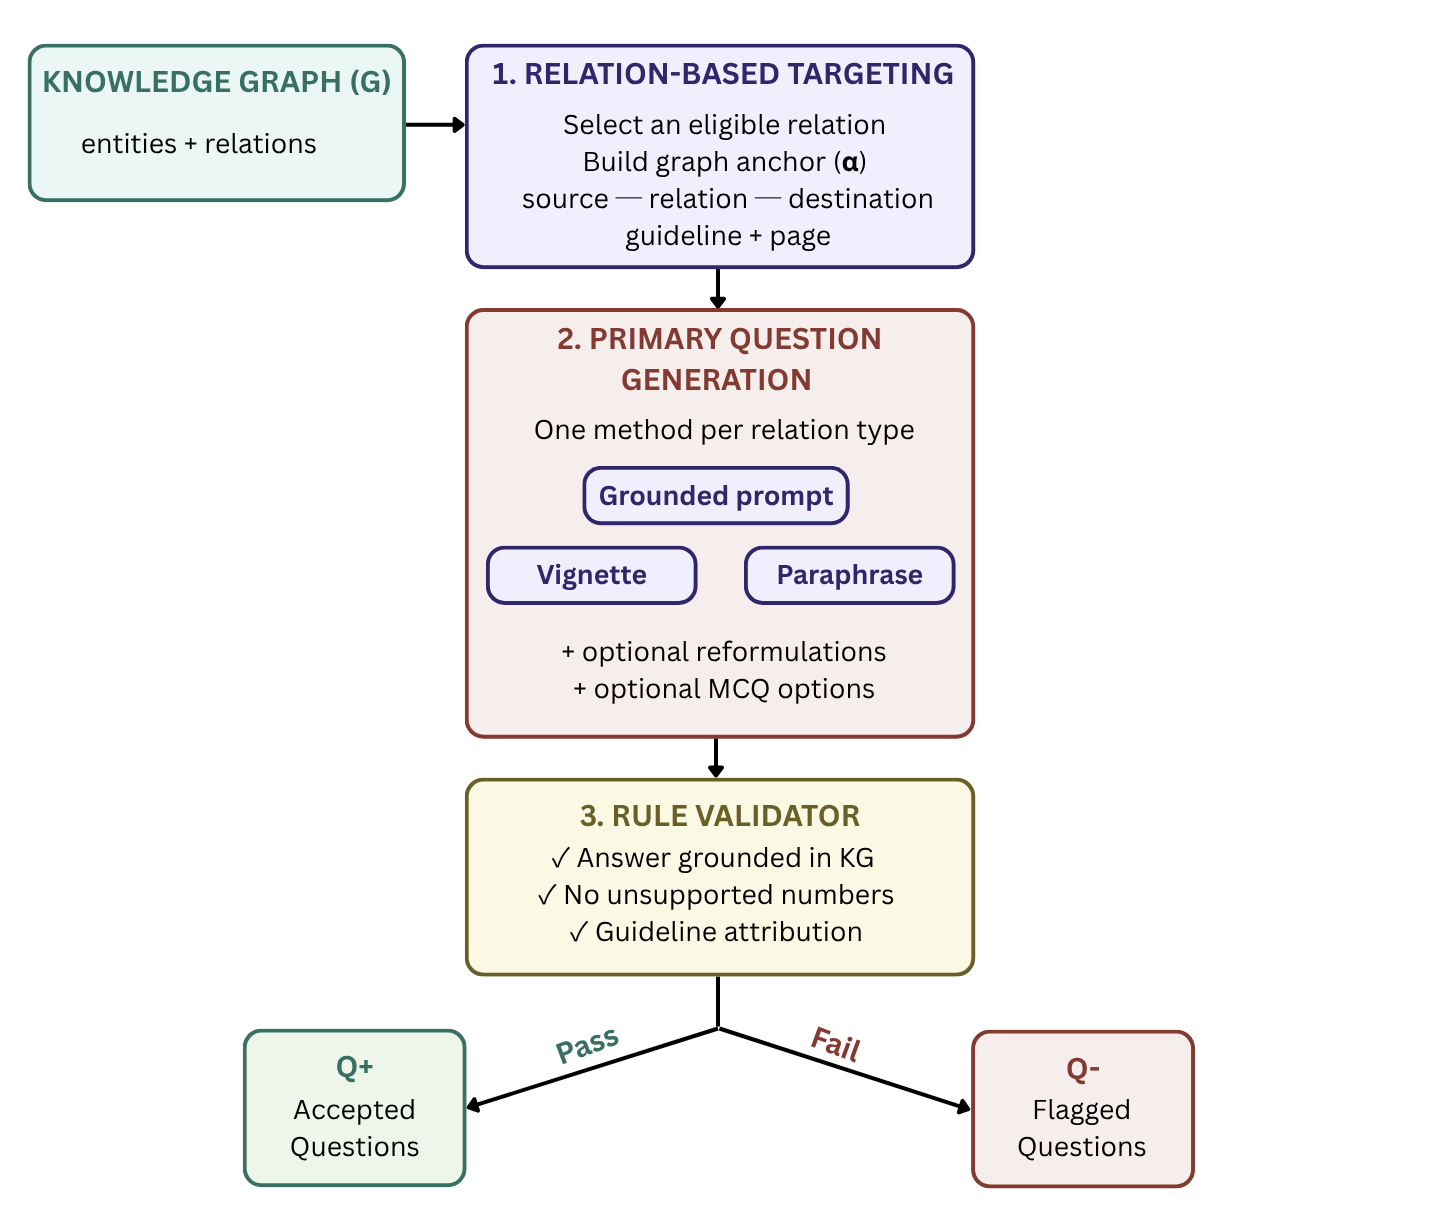
\includegraphics[width=\textwidth]{inc/figures/question_generation.png}
    \caption{Hybrid question generation pipeline.}
    \label{fig:questions}
\end{figure}

\subsection{Graph-Controlled Question Targeting}
\label{sec:targeting}

Generating questions from structured knowledge, not free text, is an established approach in question generation research \cite{guo2024,bi2020}.

The first sub-function does targeting entirely by rule-based traversal of the graph, with no language model involved.
$$\alpha: G \rightarrow \mathcal{A} \times \mathcal{D}_\gamma$$
For each edge selected, $\alpha$ produces two things. A graph anchor $a \in \mathcal{A}$ is a frozen record of the fact the question will test, carrying the source node, relation type, destination node, guideline, and page. For each selected edge, the implementation determines a question type and one primary generation method from fixed relation-based mappings. MCQ eligibility is also predefined for selected relation types, while the primary difficulty label is assigned according to the generation method

Question generation is restricted to a selected subset of graph relation types for which a meaningful question form is defined. The implementation maps each eligible relation type to a question type and generation method; for example, \textsc{first\_line\_for} maps to a \textit{which} question, \textsc{has\_target} to a \textit{what} question, \textsc{contraindicated\_in} to a \textit{yes/no} question, and \textsc{manages} to a scenario-based \textit{how} question. \textsc{equivalent\_to} edges are treated separately. They connect the same clinical concept across two guidelines, so questions derived from them test recall of one guideline's position and cross-guideline awareness at the same time.

The question taxonomy $\mathcal{T}_Q = \{\textsc{which}, \textsc{what}, \textsc{yes\_no}, \textsc{how}\}$ is decided entirely by the relation type of the anchor edge, not by the model. The mapping is a fixed lookup table set before any generation begins. \textsc{first\_line\_for} edges produce \textit{which} questions, \textsc{has\_target} edges produce \textit{what} questions, \textsc{contraindicated\_in} edges produce \textit{yes/no} questions, and \textsc{manages} edges produce scenario-based \textit{how} questions. The distribution of question types across the catalogue is a direct function of the graph's edge distribution, not of any generative choice made downstream.

\subsection{Language Model Question Formulation}
\label{sec:formulation}

The second sub-function uses a language model to produce the natural-language form of the question.
$$\beta: \mathcal{A} \times \mathcal{D}_\gamma \rightarrow \mathcal{Q}_{\text{raw}}$$
The model receives the anchor $a$ as its only factual input, given as a frozen context block, configured according to $\delta$. It is instructed not to introduce drug names, numerical values, targets, or guideline references that are absent from the anchor. In vignette-style formulations it may additionally describe the patient and symptoms in words; such details are not drawn from the anchor, and the validator checks them only for numerical values. Its intended role is therefore linguistic transformation: it may vary sentence structure, framing, and formality while preserving the factual assertion represented by the anchor.

This is a tighter version of the same constraint used during extraction. In extraction, the model was confined to a predefined schema of types and canonical names. Here, it is confined further, to the single factual assertion in one anchor. The same principle runs through both stages. Its intended role is to classify or rephrase information supplied through the structured input rather than to introduce additional clinical content.

For each anchor, the method assigned to its relation type determines how the
question is generated. The three generation methods are a graph-grounded
prompt, a clinical vignette, and a template paraphrase. For the grounded-prompt
method, the model generates one primary question, and difficulty variants may
be stored alongside it as reformulations within the same record. Each selected
anchor produces at most one primary question record in the catalogue, and exact
duplicate question texts are skipped. For relation types that support it, the
model also generates multiple-choice distractors. The correct answer is fixed
by the anchor and is never generated. For eligible multiple-choice questions,
the model is given a candidate pool sampled from real \textsc{Drug} nodes in
the graph and instructed to choose plausible distractors from that pool. This
differs from distractor generation from free text, as in \cite{gao2019}, where
distractors are generated from the passage rather than drawn from a set of
known entities. The returned strings are not programmatically checked against
the pool.

\subsection{Rule-Based Validation}
\label{sec:validation}

Language models can produce text that reads fluently but is not actually supported by their input \cite{huang2025}, so every generated question is checked against its anchor before it enters the catalogue.
$$\nu: \mathcal{Q}_{\text{raw}} \times \mathcal{A} \rightarrow \{0, 1\} \times \mathcal{Q}$$
The validator applies three checks, each comparing the generated question text against the frozen anchor.

The first check is answer-key consistency. For questions whose answer is an entity, the validator confirms that the answer named in the anchor is actually a node in the graph. For questions derived from \textsc{has\_target} edges, where the answer is a numerical threshold and not an entity name, it confirms that the number in the answer matches the property values of the destination node $v_d$ in the anchor.

The second check is hallucinated number detection. Any number in the generated question that does not appear in the anchor is flagged as a possible hallucination. This matters most for scenario-based questions, where the model can be tempted to invent realistic-sounding patient details, ages, lab values, or disease duration, that are not grounded in the anchor at all.

The third check detects conflicting guideline attribution. If the relation is associated with one of the recognised organisations, the validator rejects a question that explicitly names a different organisation. A question that credits a recommendation to the wrong organisation is factually wrong even if the recommendation content itself is stated correctly.

Questions passing all three checks go into the validated catalogue $\mathcal{Q}^+$, with anchor, generation configuration, difficulty level, and validation status recorded as metadata. Questions failing one or more checks go into a separate flagged catalogue $\mathcal{Q}^-$ for manual review. They are not discarded, since a failed check can just as easily mean the rule was too conservative as mean there is a genuine factual error. This trades some precision for recall, at the cost of needing human review on the borderline cases, which is a reasonable trade-off given that a wrong clinical claim in the catalogue actually matters. The validator checks whether the fluency and variety introduced by the language model in $\beta$ remain consistent with the content represented by the anchor in $\alpha$. What the validator checks is consistency with the anchor, not clinical correctness. A question built on an incorrect graph edge will pass all three checks, since the checks compare the question against the anchor, not against the source guideline. Chapter~\ref{chap:evaluation} reports how often this occurred in practice.

\paragraph{Worked example}
Consider an anchor in which a \textsc{Condition} node is linked by \textsc{has\_target} to a \textsc{GlycaemicTarget} representing FPG $\geq 7.0$~mmol/L. The relation also retains the organisation and page metadata associated with the extracted assertion where available. The targeting function $\alpha$ selects this relation and freezes its source node, relation type, destination node, and provenance as the anchor. The formulation function $\beta$
receives only this anchor and turns it into a question such as
``What fasting plasma glucose threshold does this guideline specify?''
The answer remains 7.0~mmol/L because it comes from the destination node,
not from the language model. The validator $\nu$ then checks the generated
question and answer against the same anchor. If the question instead
introduced a threshold of 8.0~mmol/L, the numerical check would flag it.

Figure~\ref{fig:questions} shows how the design keeps these two responsibilities separate. The left-hand annotations show the fixed mapping from relation type to question type, decided entirely by the rule engine with no language model involvement. The right-hand annotations show the range of linguistically distinct question variants the model generates from a single anchor, none of which may go beyond what the anchor specifies. The validator at the foot of the pipeline checks the generated output
against the original anchor using the three rules described above.

The composition is expressed as $(a,\delta) = \alpha(G)$, $q_{\text{raw}} = \beta(a,\delta)$, and $q = \nu(q_{\text{raw}}, a)$, making explicit that the validator $\nu$ consumes both the formulated question and the original anchor. This composed pipeline is the third contribution of this chapter. It represents question generation anchored
to the graph while keeping the factual content fixed by the selected
anchor. The factual content of each question comes from the graph in
$\alpha$. The language model in $\beta$ turns this content into natural
language, and the validator in $\nu$ checks the generated question against
the original graph assertion. The answer-bearing relation therefore remains
fixed by the anchor throughout generation. The language model contributes
the wording of the question and, where applicable, the distractor options
selected from the permitted candidate pool. This separation allows the
pipeline to produce questions with varied wording while keeping them tied
to a specific graph assertion. The concrete results of applying $\gamma$
to the graph, including question counts, type distributions, and validation
outcomes, are reported in Chapter~\ref{chap:evaluation}.
